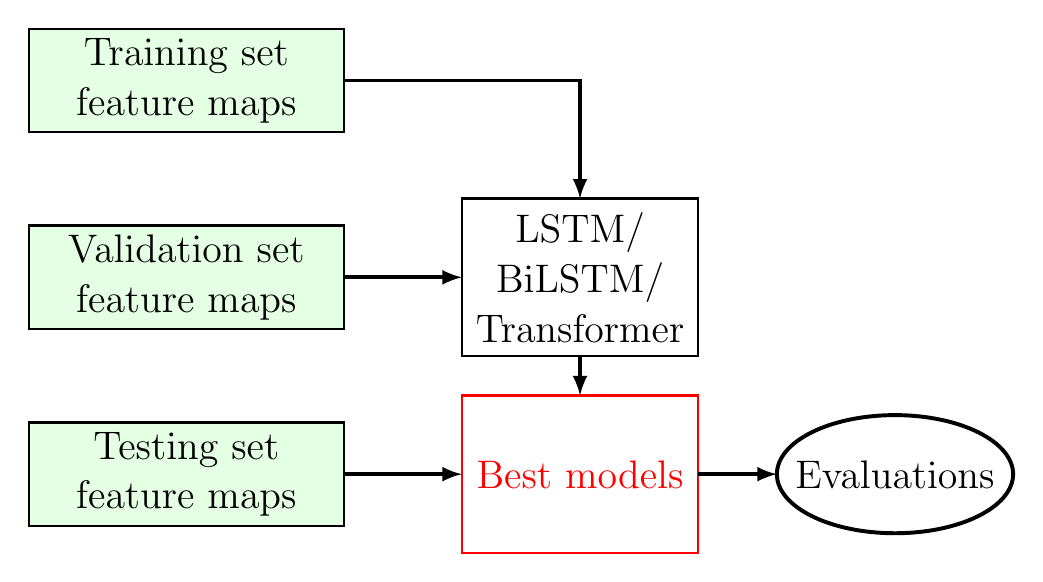
\begin{tikzpicture}[
dataset/.style={
        draw,
        line width=0.3mm,
        fill=green!10,
        minimum width=4cm,   % Your original width (1 - 0)
%         width = 1cm,
        minimum height=1cm,  % Your original height (1.5 - -2.5)
        align=center,
        font = \Large,
%         rotate=-90           % This rotates the whole box and text
    },
   model/.style = {
   draw, 
   rectangle, 
    minimum width=3cm, 
    minimum height=2cm, 
    line width = 0.3mm,
    align=center,
     font = \Large,
   },
 ]

   \node [dataset] (trainingfm) at (3,3.5) {Training set \\ feature maps};
     \node [dataset] (validationfm) at (3,1) {Validation set\\ feature maps};
     \node [dataset] (testingfm) at (3,-1.5) {Testing set\\ feature maps};

\node[model] (bestm) at (8,1) {LSTM/ \\ BiLSTM/ \\ Transformer};
% \draw[line width = 0.5mm] (6.5,0.5) rectangle (9.5,2.5) node[pos = .5, align = center] {DL model};
\draw[line width = 0.5mm, -latex] (5,1) -- (6.5,1);
\draw[line width = 0.5mm, -latex] (5,3.5) -- (8,3.5)-- (8,2);

\node[model, red] (bestm) at (8,-1.5) {Best models};
% \draw[line width = 0.5mm, red] (6.5,-2.5) rectangle (9.5,-0.5) node[pos = .5, align = center, black] {Best model};
\draw[line width = 0.5mm, -latex] (5,-1.5) -- (6.5,-1.5);
\draw[line width = 0.5mm, -latex] (8,0) -- (8,-0.5);
\draw[line width = 0.5mm, -latex] (9.5,-1.5) -- (10.5,-1.5);
\draw[line width = 0.5mm] (12,-1.5) ellipse (1.5cm and 0.75cm);
\node[align = center] at (12,-1.5) {\Large Evaluations};
% \node[align = center] at (2,3.5) {60\%};
% \node[align = center] at (2.5,1.75) {20\%};
% \node[align = center] at (2,-1) {20\%};
\end{tikzpicture}